\chapter{Ideal Gases}\label{ch:ig}

The ideal gas is one in which bombarding molecules do not exert significant forces on each other except in collisions.  Under these conditions, the distance between molecules (the gas's density) is unimportant for determining thermodynamic properties.  Only the gas's temperature (the speed of the molecules) is important.  It is worth emphasizing that transport properties (like conductivity and diffusivity) are still impacted by density.

There are two classes in \PM\ that implement the two most widely used models: the \verb|ig| class manages the Shomate equation of state, and \verb|ig2| manages the so-called NASA polynomials equation of state.  In either case, constant-pressure specific heat, $c_p$, is constructed purely as a function of temperature.  Here, we re-develop the thermodynamic properties from first principles to demonstrate how $c_p$ is sufficient to calculate them.

\section{Properties of ideal gases}

\subsection{Ideal gas law}

When they are spread so sparsely that forces between molecules are small, ideal gases are well described by the relations
\begin{subequations}
\begin{align}
p &= n k T\label{eqn:ig:k}\\
p &= \rho R T\label{eqn:ig:r}\\
p &= \overline{\rho} R_u T\label{eqn:ig:ru}.
\end{align}
\end{subequations}
Here, $p$ and $T$ are the pressure and temperature of the gas.  The densities are expressed in number density, $n$, mass density, $\rho$, and molar density, $\overline{\rho}$.  It is clear, then, that the Boltzmann constant, $k$, and the ideal gas constants, $R$ and $R_u$, are related,
\begin{align}
k N_a = R W = R_u.
\end{align}
The Boltzmann constant is integral to the fundamental definition of the units of temperature (see Section \ref{sec:units:temperature}), so this relationship makes it possible to calculate the universal gas constant in molar units and the ideal gas constant in mass units.

This law is empirical in its origins.  It was originally formulated as an amalgamation of the independent laws of Gay-Lussac, Charles, and Boyle.  The kinetic theory of gases eventually provided an independent formulation based entirely in Newton's laws.  Given its importance to the study of matter and its deeply intuitive nature, it is surprising that virtually no introductory text on thermodynamic gives the subject any treatment.  It is worth a brief summary here.

First, let us take that a gas is comprised of molecules that translate freely in space.  They may be imagined to follow straight paths of constant velocity unless they collide with a containing wall or another molecule.  

Pressure, then, is due to a near continuous stream of impacts on a surface.  It only has meaning when the density of molecules is sufficiently high that their individual impacts are imperceptible.  Pressure, then, is a kind of average force determined by a series of may individual random impacts.  It is possible to quantify its magnitude by describing the individual imapcts through Newtonian mechanics.  If the forces due to a series of impacts in time is $F(t)$, a surface with area, $A$, will experience a pressure, $p$, based on the rate of increase of total impulse,
\begin{align}
p \equiv \frac{1}{A t} \int_0^t F(\tau) \d \tau.
\end{align}
This definition should have a well defined value in the limit where $t$ is larger than period between individual impacts.

In a Cartesian coordinate system with $z$ normal to a surface and positive \emph{into} the surface, the velocity of any single molecule will have three components, $\vec{u}_1 = u_x \hat{i} + u_y \hat{j} + u_z \hat{k}$.  After an elastic collision with the surface, the velocity will be $\vec{u}_2 = u_x \hat{i} + u_y \hat{j} - u_z \hat{k}$.

The impulse imparted to the surface by one such collision will be
\begin{align}
\int_0^t F \d \tau = 2 m u_z,
\end{align}
when $m$ is the mass of the molecule.  When collisions occur due to many identical molecules, their impulses accumulate
\begin{align}
\int_0^t F \d \tau &= 2 m \left( u_{z,1} + u_{z,2} + u_{z,3} + \ldots \right)\nonumber\\
  &= 2 m \sum_i u_{z,i}
\end{align}
Note that for a molecule to collide with the surface, its $z$-component velocity before the collision, $u_z$, must be positive.  This results in a purely positive force (into the surface).  Ideal gas molecules experiencing elastic collisions have no mechanism to pull on the surface.

The next step to predict the force on the surface requires a prediction for the rate at which  collisions occur.  Because faster moving molecules will travel more distance in the time interval, their collisions will be more numerous.  Let the number density of molecules with $z$-component velocity between $u_z$ and $u_z + \d u_z$ be $n'(u_z) \d u_z$.  Here, $n'$ is a population density function for a population of molecules based on one component of their velocity.  So, $n'$ has units number per volume per velocity, and its integral over all velocities is precisely $n$, the total number density of molecules.

The number of molecules with a certain velocity that will strike an area, $A$, in time $t$ will be determined by the size of the volume that can be traversed by molecules traveling at that velocity.  Molecules traveling with $z$-component velocity $u_z$ will traverse a length $u_z t$ in the time interval.  So, the total volume occupied by molecules with that velocity that will strike the surface is $A t u_z$.  The total number of collisions is $A t u_z n'(u_z) \d u_z$.  So, the impulse becomes
\begin{align}
\int_0^\tau F \d \tau &= 2 m \int_0^{\infty} A t u_z{^2} n'(u_z) \d u_z\nonumber
 &= m A t \int_{-\infty}^\infty u_z{^2} n'(u_z) \d u_z
\end{align}
Note that only half of the gas's population will have a velocity component in the positive direction, and the other half will not cause pressure.  Therefore, the 2 coefficient is canceled when the bounds of the integral are extended to include all molecules.

The integral is merely a calculation of the average value of $u_z{^2}$ over the population of molecules, and may be simplified to $n \langle u_z{^2} \rangle$ when $n$ is simply the total number density of the molecules and $\langle u_z{^2} \rangle$ is the mean square of $z$-component velocity.  Finally, we have obtained an expression for pressure in terms of the outward velocity component,
\begin{align}
p = m n \langle u_z{^2}\rangle.
\end{align}

The last simplification to this relationship comes when we assert that gas velocity statistics are isotropic; velocity statistics are the same in all directions and do not depend on the coordinate system.  That implies that $\langle u_x{^2} \rangle = \langle u_y{^2} \rangle = \langle u_z{^2} \rangle$, so
\begin{align}
\langle \vec{u}^2\rangle = \langle u_x{^2} + u_y{^2} + u_z{^2} \rangle = 3 \langle u_z{^2} \rangle.\label{eqn:ig:3dof}
\end{align}
Therefore, pressure is proportional to the mean square of molecular translational velocity,
\begin{align}
p = 3 m n \langle u{^2} \rangle.
\end{align}
When this relationship is substituted into the ideal gas law above, it provides a purely mechanical interpretation for temperature as well,
\begin{align}
\langle \frac{1}{2} m u{^2} \rangle = \frac{3}{2} k T.\label{eqn:thermal:k}
\end{align}
Temperature is a measure of the average \emph{thermal} energy of the gas.  Higher temperature means higher kinetic energy, and the Boltzmann constant relates the two.

This development was quick and it neglects to address mixtures of molecules of different masses.  However, the same approach may be used quite intuitively to show that Dalton's law for partial pressures also follows from these basic assumptions.

\subsection{Internal energy}

What happens to heat and work as they are added to an ideal gas depends on the structure of the gas molecule.  If there are chemical, atomic, or phase changes, the species can be modeled as vanishing and being replaced by a new substance with its own properties.  The ideal property models are, therefore, concerned with how energy is stored in a molecule that is neither changing its fundamental structure nor changing phase.  This remaining energy will be exhibited entirely as the thermal energy in (\ref{eqn:thremal:k}) and internal vibration, rotation, or electrical motions inside the molecule, for which we have not yet accounted.

{\bf Perfect gases} are ideal gases, but not all ideal gases are perfect.  The molecules of an ideal gas collide elastically and have no further interactions with their surroundings.  However, the molecules of a perfect gas are further assumed to neither spin nor vibrate.  As a result, any molecule more complicated than a single atom does not form a perfect gas.

When a gas composed of a monoatomic molecule like argon is heated (without atomic, chemical, or phase changes) the energy can only be stored in the thermal translational energy described in (\ref{eqn:thermal:k}).  A sample of $N$ molecules of such a gas would have thermal energy $N \frac{3}{2} k T$, so the energy per mole is
\begin{align}
e - e_0 &= \frac{N_a}{W} \frac{3}{2} k T = \frac{3}{2} R T \label{eqn:pg:e}
\end{align}
when $e_0$ is the internal energy due to the atomic, chemical or phase changes we have not yet considered.  Note that when this is expressed in molar units, $R$ becomes $R_u$, and when it is expressed in molecules, $R$ is replaced by the Boltzmann constant, $k$.

{\bf Non-perfect ideal gases} are made of more complicated molecules can store energy in more complicated ways; they vibrate, they rotate (spin), and they have means of storing energy electrically.  They do this because the can; they have more degrees of freedom.

The 3 in (\ref{eqn:pg:e}) first appeared in (\ref{eqn:ig:3dof}) because all ideal gases are free to translate in three directions.  These three thermal degrees of freedom are the only ones that contribute to measurements of temperature, but complex molecules have more degrees of freedom.  If these are included in the internal energy as well, a molecule that is free to vibrate, rotate, and translate in $f$ degrees of freedom will have an internal energy
\begin{align}
e - e_0 &= \frac{N_a}{W} \frac{f}{2} k T = \frac{f}{2} R T.
\end{align}

The intuitive assumption might be that $f$ is constant and a property of each molecule.  This assumption implicitly asserts that all modes of vibration, rotation, and translation have an equal fraction of the total energy so it is called the \emph{equipartition} assumption.  It results in an elegant formulation, but it completely fails to predict the actual behavior of molecules in gases.

Instead, it is necessary to stipulate that $f$ is a statistical quantity that can change with the state.  It can be thought of as the number of ``active'' degrees of freedom of each molecule.  Its minimum is 3, but it can increase to a maximum that will depend on the complexity of the molecule and the energy of the collisions it endures.  For example, at very low temperatures, molecules may not vibrate much; instead they may just bang around and spin like rigid bodies (see Figure \ref{fig:dof} below).  However, at higher temperatures, there may be enough energy to excite vibrations inside the molecules.

Fortunately, since all ideal gases (perfect or not) are presumed to collide elastically, the equilibrium distribution of energy should depend on neither the rate of collisions nor the distance separating the molecules.  Obviously, this assumption will break when molecules are packed in closely with one another.  However, so long is that is true, the active degrees of freedom and the internal energy will both only be a function of temperature (the average kinetic energy).
\begin{align}
e(T) - e_0 = \frac{f(T)}{2} R T \label{eqn:ig:e}
\end{align}

Better insights into the behavior of $f$ will be seen when we examine specific heats below.

\subsection{Enthalpy}

As established above, we will construct all of the properties of the ideal gas in terms of its specific heat, but in order to derive reliable relations for the specific heats, it is important to first re-examine enthalpy.

Recall from Section \ref{sec:intro:h} that the definition for enthalpy is $e + pv$.  For an ideal gas, $pv$ may be substituted for $R T$, so an ideal gas will have enthalpy
\begin{align}
h(T) = e(T) + RT.\label{eqn:ig:h}
\end{align}

For all ideal gases, enthalpy and internal energy are only functions of temperature, and they are related by $RT$.

\subsection{Specific heats}

Recall from Section \ref{sec:intro:c} that the constant-volume and constant-pressure specific heats are
\begin{align}
c_v &= \left( \frac{\partial e}{\partial T} \right)_v\nonumber\\
c_p &= \left( \frac{\partial h}{\partial T} \right)_p\nonumber
\end{align}

Because both internal energy and enthalpy are only functions of temperature, this relationship is relatively simple,
\begin{align}
c_v &= \frac{f(T)}{2} R \left( 1 + T\frac{f'(T)}{f(T)}\right) \approx \frac{f(T)}{2} R \label{eqn:ig:cv}\\
c_p &= c_v + R\label{eqn:ig:cp}.
\end{align}

The approximation in (\ref{eqn:ig:cv}) only holds when $f(T)$ is very nearly constant. 

Figure \ref{fig:dof} shows the quantities $2 c_v / R$ for six gases with increasing molecular complexities.  The perfect gases, He and Ar, behave precisely as predicted with exactly three degrees of freedom.  All four polyatomic molecules start with quasi-rigid motion at low temperatures before adopting higher degrees of freedom at high temperatures.

\begin{figure}
\centering
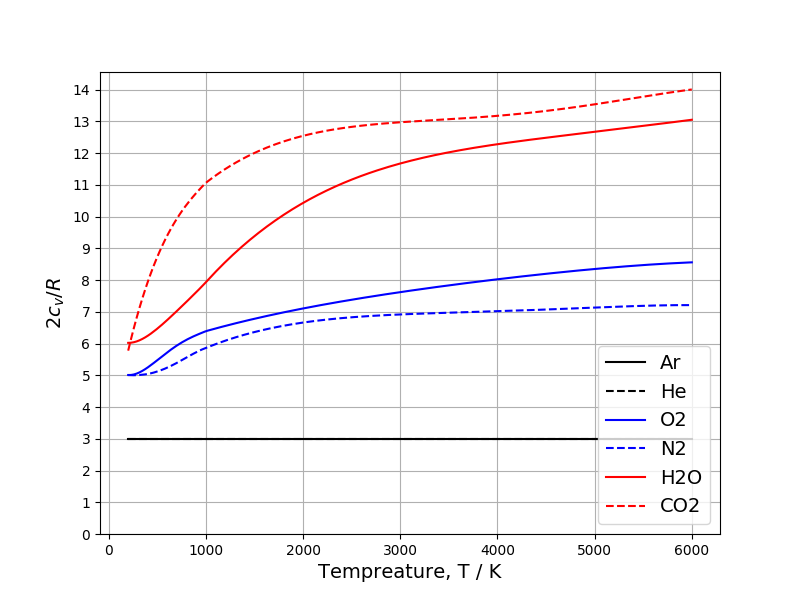
\includegraphics[width=0.97\textwidth]{figures/dof}
\caption{Approximate mean active degrees of freedom in selected ideal gas models}\label{fig:dof}
\end{figure}

For H$_2$O, rigid motion means six degrees of freedom: three coordinates of translation and three axes of rotation.  For diatomics like O$_2$ and N$_2$, however, their symmetry robs them of one of their axes of rotation, so they only exhibit five degrees of freedom at low temperatures.  Since CO$_2$ is also an axisymmetric molecule, it can be seen asymptotically approaching 5 at low temperatures as well.

\subsection{Entropy and enthalpy revisited}

Recall from Section \ref{sec:intro:s} that the entropy of any substance changes like
\begin{align}
T \d s = \d h - v \d p\nonumber.
\end{align}
For the ideal gas, this can be simplified by substituting $R T / p$ for $v$ and integrating to obtain
\begin{align}
s - s_0 = \int c_p(T)\frac{\d T}{T} - \int R \frac{\d p}{p}\label{eqn:ig:s}.
\end{align}
For a perfect gas,
\begin{align}
s - s_0 = c_p \ln\left( \frac{T}{T_0} \right) - R \ln\left( \frac{p}{p_0} \right)\label{eqn:pg:s}.
\end{align}

An identical approach can be taken for enthalpy, but with an even simpler result.  
\begin{align}
h - h_0 = \int c_p(T) \d T
\end{align}
For a perfect gas,
\begin{align}
h - h_0 = c_p \left(T - T_0\right).
\end{align}

The ideal gas classes in \PM\ use systems of coefficients to form piece-wise polynomials for $c_p(T)$ to match empirical data.

\section{Other properties}

Once $c_p(T)$ and $h(T)$ are well defined, it is also possible to evaluate internal energy,
\begin{align}
e(T) = h(T) - RT,
\end{align}
constant-volume specific heat,
\begin{align}
c_v(T) = c_p(T) - R,
\end{align}
specific heat ratio,
\begin{align}
\gamma(T) = \frac{c_p(T)}{c_p(T) - R},
\end{align}
speed of sound
\begin{align}
a(T) = \sqrt{\gamma(T) R T},
\end{align}
and others.

The central problem, then, is how to calculate $c_p(T)$.

As becomes clear in the next sections, polynomials are important to these formulations; so much so that we devote a separate section to their efficient evaluation.

\section{The ideal gas classes}

\subsection{The Shomate equation: \texttt{ig1}}

\PM's IG1 class is built on the Shomate equation for constant-pressure specific heat $c_p$.  This is the formulation used by the NIST/JANAF thermophysical property database.

The Shomate equation takes the form
\begin{align}
t &= \frac{T}{T_s}\\
c_p(t) &= c_0 + c_1 t + c_2 t^2 + c_3 t^3 + \frac{c_4}{t^2},
\end{align}
where the scaling temperature, $T_s$ is 1000K for all species.  Reducing the argument to the polynomial, $t$, to by on the order of 1 is an intelligent step to help reduce numerical errors, but it should be obvious that there is no attempt to base the formulation on fundamental physics.  This is a purely empirical formula.  Physics-based expressions for the specific heat of gases are available, but they become so numerically cumbersome, equations as simple as these are far preferable when available.

Because of its simplicity, the Shomate equations lacks the degrees of freedom to express specific heat over wide ranges, so data are usually given in piece-wise formulations.  For example, tungsten dioxide (WO$_2$), has a set of coefficients for $298\mathrm{K} \le T < 1100\mathrm{K}$ and $1100\mathrm{K} \le T \le 6000\mathrm{K}$.

The enthalpy can be explicitly calculated from (\ref{eqn:ig:enthalpy}),
\begin{align}
h(T) &= h_0 + \int c_p(T) \d T \nonumber\\
 &= h_0 + T_s \int c_p(t) \d t \nonumber\\
 &= T_s \left(c_0 t + \frac{c_1}{2} t^2 + \frac{c_2}{3} t^3 + \frac{c_3}{4} t^4 - \frac{c_4}{t} + c_5 \right).
\end{align}
It is important to emphasize that $h_0$ is not the same as the enthalpy of formation, $\Delta h^\circ_f$.  Instead, it is merely an integration constant, which can be alternately expressed as a new coefficient, $c_5$.

Because of the temperature term in the denominator, no multiple of $T_s$ appears in entropy when the integration is changed to $t$,
\begin{align}
s(T,p) &= s^\circ(T_{ref}) + \int_{T_{ref}}^T \frac{c_p(\tau)}{\tau}\d \tau - R \ln \left( \frac{p}{p_{ref}} \right)\nonumber\\
 &= s^\circ(T_{ref}) + \int_{T_{ref}}^T \frac{c_p(\tau)}{\tau}\d \tau - R \ln \left( \frac{p}{p_{ref}} \right)\nonumber\\
s(T,p) &= c_0 \ln t + c_1 t + \frac{c_2}{2} t^2 + \frac{c_3}{3} t^3 -\frac{c_4}{2t^2} + c_6 - R \ln\left(\frac{p}{p_{ref}}\right).
\end{align}
Just like in the enthalpy integral, a new coefficient, $c_6$, has been introduced to represent the integration constant.

Internal energy is readily calculated from the definition of enthalpy in (\ref{eqn:enthalpy}),
\begin{align}
e(T) &= h(T) - RT\nonumber\\
\end{align}
There is a similarly simple relationship to determine constant-volume specific heat and specific heat ratio,
\begin{align}
c_v(T) &= c_p(T) - R\\
\gamma(T) &= \frac{c_p(T)}{c_p(T)-R}
\end{align}

\subsection{The NASA polynomial: \texttt{ig2}}

Like the Shomate equation, the NASA polynomials are a piece-wise empirical formulation to the specific heat of an ideal gas.  Unlike the Shomate equation, there is no $1/t^2$ term, they make no attempt to scale temperature prior to evaluating the polynomial, and they are scaled with respect to the species' ideal gas constant.

\begin{align}
c_p(T) = R\left(c_0 + c_1 T + c_2 T^2 + c_3 T^3 + c_4 T^4\right)
\end{align}

There are nearly identical formulations for enthalpy,
\begin{align}
h(T) = R \left(c_0 T + \frac{c_1}{2} T^2 + \frac{c_2}{3} T^3 + \frac{c_3}{4} T^4 + \frac{c_4}{5}T^5 + c_5 \right),
\end{align}
and entropy
\begin{align}
s(T) = R \left(c_0 \ln(T) + c_1 T + \frac{c_2}{2} T^2 + \frac{c_3}{3} T^3 + \frac{c_4}{4} T^4 + c_6\right).
\end{align}
Here, just as in the Shomate equations, $c_5$ and $c_6$ are introduced as integration constants in enthalpy and entropy.

Internal energy is readily calculated from the definition of enthalpy in (\ref{eqn:enthalpy}),
\begin{align}
e(T) &= h(T) - RT\nonumber\\
\end{align}
There is a similarly simple relationship to determine constant-volume specific heat and specific heat ratio,
\begin{align}
c_v(T) &= c_p(T) - R\\
\gamma(T) &= \frac{c_p(T)}{c_p(T)-R}
\end{align}

\section{Enthalpy of formation, $\Delta_f h^\circ$}

The species in the \PM\ ideal gas collection all obey this convention, so that they are suitable for models with chemical reactions with one another.  The species in the multi-phase collection, however, are not.  Chemical reactions require that more than one molecule is present, but the multi-phase models are specifically tuned to the intermolecular forces of a pure substance.  Since the mixtures required for chemical reactions would break the multi-phase models anyway, there is no need to deal with the added complexity of consistent reference states for chemical reactions.

For ideal gases, the reference state is defined by convention established in the NIST-JANAF Thermochemical Tables \footnote{Malcom Chase, \emph{NIST-JANAF Thermochemical Tables Fourth Edition}, National Institute of Standards and Technology, 1998.}.  They are $T_{ref} = $ 298.15K (25$^\circ$C) and $p^\circ = $ 1bar.  It should be emphasized that these reference conditions are not universally adopted in other fields of study.  For example, reports in gas metrology usually use 1atm and 0$^\circ$C.

After a sufficiently detailed study of the isobaric specific heat, the enthalpy of an ideal gas is, therefore,
\begin{align}
h^circ(T) = \Delta_f h^\circ(T_{ref}) + \int_{T_{ref}}^T c_p^\circ(T) \d T.
\end{align}
As indicated by the $^\circ$ super-scripts, this calculation is performed at reference pressure.  A discussion of pressure dependence is left for the ideal gas chapter.

The species in question is constructed by a sequence of chemical reactions from certain reference species (e.g. H$_2$O is constructed from H$_2$ and O$_2$) and that reaction can be determined to have an enthalpy of formation by experiment.

While \PM\ is not careful to identify reference species, the source from which the models are taken is.  By convention, the common diatomic gases all have zero enthalpy of 
